\documentclass[11pt,letterpaper]{article}
\usepackage[utf8]{inputenc}
\usepackage{geometry}
\usepackage{tikz}
\usetikzlibrary{arrows.meta,positioning}

\geometry{letterpaper, left=1in, right=1in, top=0.75in, bottom=1in}

\begin{document}

\thispagestyle{empty}

% Rule R-30: Top Margin Drawing Identification
\noindent
\begin{minipage}{\textwidth}
\raggedleft
\footnotesize\fontfamily{phv}\selectfont
Application No.: 19/561,236 \quad Sheet 1 of 1 \quad Inventor: Reinaldo Javier Aguiar Marcano \quad \textbf{Replacement Sheet}
\end{minipage}

\vspace{1.5cm}

\begin{center}
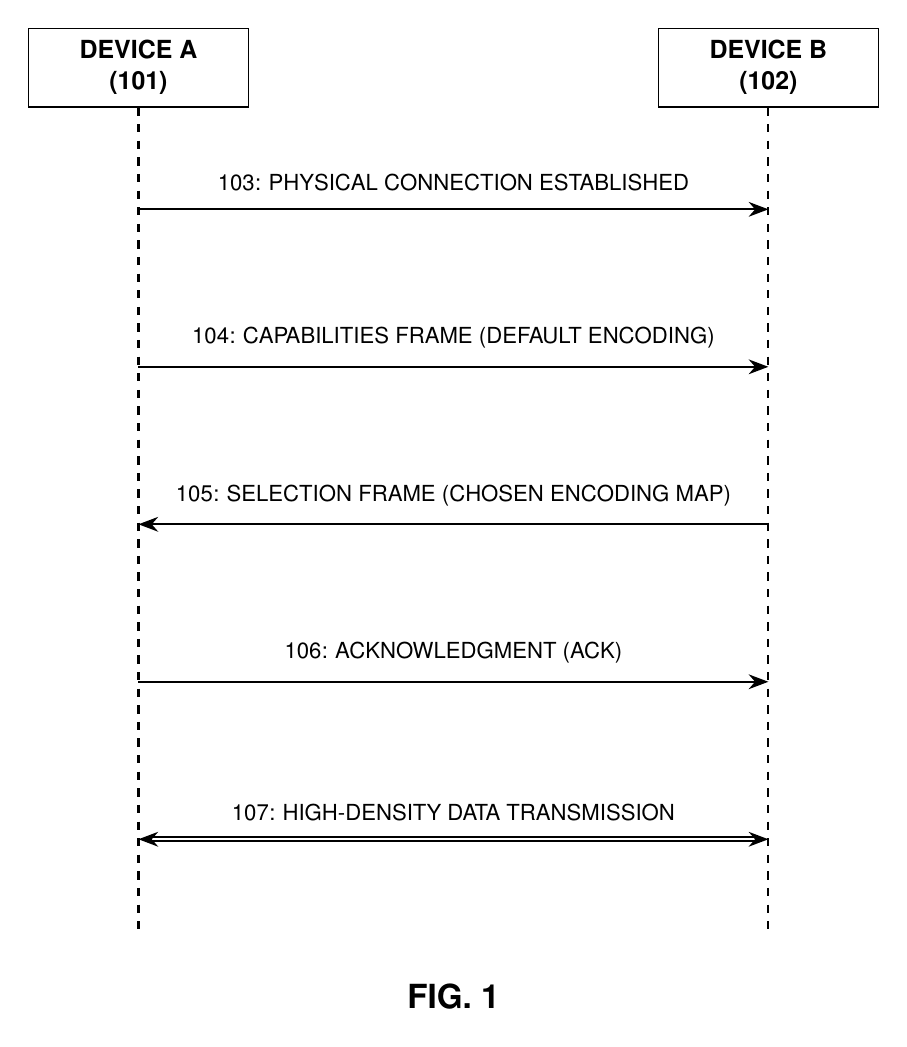
\begin{tikzpicture}[
    box/.style={draw, rectangle, minimum width=2.8cm, minimum height=1.0cm, align=center, font=\fontfamily{phv}\bfseries\small},
    arrow/.style={-{Stealth[length=2.5mm]}, thick},
    label/.style={font=\fontfamily{phv}\footnotesize, align=center}
]

% Devices
\node[box] (devA) at (0, 0) {DEVICE A\\(101)};
\node[box] (devB) at (8, 0) {DEVICE B\\(102)};

% Lifelines
\draw[dashed, thick] (devA.south) -- (0, -11.0);
\draw[dashed, thick] (devB.south) -- (8, -11.0);

% Sequence Messages
% Step 103: Physical Connection
\draw[arrow] (0, -1.8) -- (8, -1.8) node[midway, above=1mm, label] {103: PHYSICAL CONNECTION ESTABLISHED};

% Step 104: Capabilities Frame
\draw[arrow] (0, -3.8) -- (8, -3.8) node[midway, above=1mm, label] {104: CAPABILITIES FRAME (DEFAULT ENCODING)};

% Step 105: Selection Frame
\draw[arrow] (8, -5.8) -- (0, -5.8) node[midway, above=1mm, label] {105: SELECTION FRAME (CHOSEN ENCODING MAP)};

% Step 106: Acknowledgment
\draw[arrow] (0, -7.8) -- (8, -7.8) node[midway, above=1mm, label] {106: ACKNOWLEDGMENT (ACK)};

% Step 107: Data Transmission
\draw[{Stealth[length=2.5mm]}-{Stealth[length=2.5mm]}, double, thick] (0, -9.8) -- (8, -9.8) node[midway, above=1mm, label] {107: HIGH-DENSITY DATA TRANSMISSION};

% Figure Label
\node[font=\fontfamily{phv}\bfseries\large] at (4, -11.8) {FIG. 1};

\end{tikzpicture}
\end{center}

\end{document}
